\documentclass{jsarticle}

 \usepackage{ascmac}
 \usepackage{graphicx}
 \usepackage[dvipdfmx]{color}
 \usepackage{amssymb,amsmath,amsthm}
 \usepackage{graphics}
 \usepackage{fancybox, tcolorbox}
 \tcbuselibrary{raster,skins, breakable}
 \usepackage{nccmath}
 \usepackage{tikz}
 \usetikzlibrary{intersections, calc, cd}
 \usepackage{bm}
 \usepackage[italicdiff]{physics}
 \usepackage{titlesec}
 \usepackage{mathtools}
 \usepackage{enumerate}
 \usepackage{float}

 \numberwithin{equation}{section}
 \setcounter{tocdepth}{3}

\title{{Variance Sum Rule for entropy production のメモ \\[2ex]\large 最終更新日: \today}}
\author{八木俊輔}
\date{}

\theoremstyle{definition}

\newcommand{\ave}[1]{\langle #1 \rangle}

\usepackage{fancyhdr}
\pagestyle{fancy}
    \lfoot{}
    \cfoot{\thepage}
    \rfoot{}

\begin{document}
\maketitle
\tableofcontents
\clearpage

\newpage 
\section{要約}
エントロピー生成は非平衡物理学の特徴であり,不可逆性,散逸,およびエネルギー変換プロセスの効率を定量化する.
これまでの多くの試みにもかかわらず,ナノスケールでのエントロピー生成の測定は依然として困難である.
そこで我々は,変位と力の分散に対する分散和則(VSR)を導入し,それによって非平衡定常状態におけるエントロピー生成率を測定することが可能にした.
まず,光トラップ内のアクティブブラウン運動粒子など,直接測定可能な力に対して VSR を説明する.
次に,ヒト赤血球の揺らぎ実験に VSR を適用する.その結果,測定された $\sigma $ は空間的に不均一であり,有限の相関長を持つことが分かった.
また,その平均値は熱量測定の結果と一致した.
VSRは,生体およびアクティブマターにおける力スペクトロスコピーや時間分解イメージングを使用して, $\sigma $ を導出するための道を開く.

\section{イントロダクション}
非平衡定常状態(NESS)は,気候ダイナミクス,生細胞,アクティブマターに至るまで,自然界に広く存在する.
その状態の基本的な量として,エネルギーが環境に散逸する速度であるエントロピー生成率 $\sigma$ が挙げられる.
これは熱力学の第2法則により正であることが保証されている.
エントロピー生成の測定はその重要性にもかかわらず依然として難しく,特に確率的で空間的に変動する揺らぎや,微視的変数へのアクセスが制限される微視的システムにおいては困難である.
エントロピー生成率 $\sigma $ は,古典および量子系におけるエネルギー変換効率,生細胞のエネルギーコストや不可逆な挙動を決定する.
力や流れが実験的にアクセスできない場合,$\sigma $は捉えにくい量である.
時間の不可逆性,熱力学的不確実性関係,および粗視化,から不等式を得ることはできるが,これらの結果の多くは,熱力学第2法則よりも強い制限をするだけに留まり,$\sigma \geq 0$ を保証するものの,しばしば上限がなく実際の $\sigma$ についての有益な情報を提供しない.
ナノスケールにおける散逸プロセスをより正確に評価するためには, $\sigma $ を推定するための代替的な方法が必要である.

\newpage 
\section{Variance Sum Rule}
まずは Variance Sum Rule (VSR) を導入する.
ここでは NESS にプローブ粒子が接しているような状況を考える(図1).

\begin{figure}[H]
  \begin{center}  
  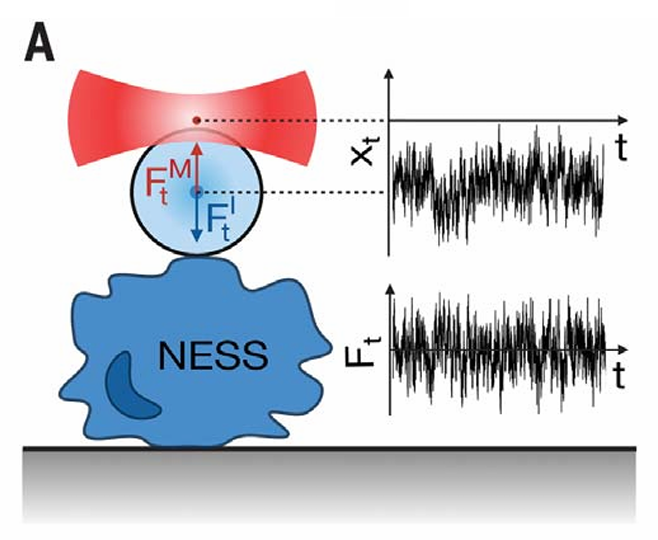
\includegraphics[width=5cm]{vsr_fig1a.png}  
  \end{center}
  \caption{考えている状況}
\end{figure}

粒子の運動は,つぎの Langevin 方程式で記述される.
\begin{equation}
  \dot{x}(t) = \mu F(t) + \sqrt{2D} \eta(t)
\end{equation}
$\mu $は移動度で,$D$はノイズの強さを決定する拡散係数,$\eta (t)$は白色ノイズ \footnote{白色ノイズとは@@@} である.
$F(t)$は粒子に働く力であり,それは測定機械が及ぼす力 $F^M (t)$と,系の内部で起こる力 $F^I (t)$ の和である.
\begin{equation}
  F(t) = F^M (t) + F^I (t)
\end{equation}
これも図1に示してある.
多くの実験では,$F^I (t)$が測定できないため,エントロピー生成率 $\sigma $は直接測定することができない.\\
\quad ここでは単位時間当たりに熱 $Q(t)$ がどの程度散逸するのかを,その分散 $\mathcal{V} _Q (t) = \langle Q(t)^2 \rangle - \langle Q(t) \rangle^2 $ によって定量化する方法をとる.
ここで $\langle \cdot \rangle $ はNESSにおける動的平均\footnote{時間平均の意味でとって構わない.}を表す.\\
\quad ここから VSR を導出する.まずは簡単のため1次元で行い,系は温度 $T$ の熱浴に接しているとする.
白色ノイズの性質より,つぎが成り立つ.
\begin{equation}
  \ave{\eta (t)} = 0
\end{equation}
\begin{equation}
  \label{gauss_2}
  \ave{\eta (t) \eta(t')} = \delta (t-t')
\end{equation}
拡散係数と移動度との間には,つぎのような関係がある.
\begin{equation}
  D = k_B T \mu
\end{equation}
簡単のために $F(t)$ はつぎのようにかけるものとする.
\begin{equation}
  F(t) = - \pdv{U(x(t) - \lambda (t))}{x}
\end{equation}
ここで $\lambda (t)$ は前もって決められたプロトコルに従って動く変数である.
また,ここでは周期的に変化する NESS などは考えず,時間変動のない NESS のみを考える.\\
\quad 準備のために,相関関数についても触れておく.2つの可観測量 $A(t), B(t)$ についての(連結)相関関数は,
\begin{equation}
  C_{AB} (t) = \ave{A(t) B(0)} - \ave{A(0)} \ave{B(0)}
\end{equation}
と定義される.また,今考えているNESSでは
\begin{equation}
  \label{NESS}
  \ave{A(t)} = \ave{A(0)}
\end{equation}
であって,これは時間に依存しない.\\
\quad ここから VSR を導出する.まずは,先に示した Langevin 方程式を $0 \to t$ で積分する.
\begin{equation}
  \label{Langevin}
  \dot{x}(t) = \mu F(t) + \sqrt{2D} \eta(t)
\end{equation}
\begin{equation}
  x(t) - x(0) = \mu \int_0^t F(s) ds + \sqrt{2D} \int_0^t \eta(s)ds
\end{equation}
\begin{equation}
  \Delta x(t) - \mu \int_0^t F(s) ds = \sqrt{2D} \int_0^t \eta(s)ds \quad (\Delta x(t) := x(t) - x(0))
\end{equation}
これを2乗する.
\begin{equation}
  \qty{ \Delta x(t) } ^2 + \mu^2 \qty{\Sigma_F (t)} ^2 - 2\mu \Delta x(t) \int_0^t F(s) ds = 2D \int_0^t \int_0^t \eta(s) \eta(s') dsds'
\end{equation}
ただし,ここで $\Sigma_F (t) := \int_0^t F(s) ds$ である.式 (\ref{gauss_2}) より,
\begin{equation}
  \label{totyu1}
  \qty{ \Delta x(t) } ^2 + \mu^2 \qty{\Sigma_F (t)} ^2 = 2\mu \Delta x(t) \int_0^t F(s) ds + 2Dt
\end{equation}
となる.ここで,便利のために幾つかの物理量を導入する.\\
\quad まずは分散を考える.定義より,
\begin{equation}
  \mathcal{V} _{\Delta x} (t) = \langle \qty{ \Delta x(t) } ^2 \rangle - \langle \Delta x(t) \rangle^2
\end{equation}
\begin{equation}
  \mathcal{V} _{\Sigma_F} (t) = \langle \qty{ \Sigma_F (t) } ^2 \rangle - \langle \Sigma_F (t) \rangle^2
\end{equation}
である.ここで,式(\ref{Langevin}) の両辺で時間平均をとれば,容易に
\begin{equation}
  \langle \Delta x(t) \rangle^2 = \mu^2 \langle \Sigma_F (t) \rangle^2
\end{equation}
が分かる.さらに,式 (\ref{NESS}) より
\begin{equation}
  \langle \Delta x(t) \rangle = \langle \Delta x(0) \rangle = 0
\end{equation}
であるので,分散は
\begin{equation}
  \mathcal{V} _{\Delta x} (t) = \langle \qty{ \Delta x(t) } ^2 \rangle
\end{equation}
\begin{equation}
  \mathcal{V} _{\Sigma_F} (t) = \langle \qty{ \Sigma_F (t) } ^2 \rangle
\end{equation}
となる.\\
\quad 続いて相関関数について考える.相関関数の差は,つぎのようになる.
\begin{equation}
  \label{sokan1}
  C_{xF} (s) - C_{Fx} (s) = \langle x(s)F(0) \rangle - \langle F(s)x(0) \rangle
\end{equation}
この右辺第一項に $2 \mu$ をかけて, $0 \to t$ で積分し,変形をしておく.
\begin{align}
  2\mu \int_0^t \langle x(s)F(0) \rangle  ds &= 2\mu \int_t^0 \langle x(t - s')F(0) \rangle  (-ds') \\
  &= 2\mu \int_0^t \langle x(t)F(s') \rangle ds' \quad \text{(相関関数は時刻をずらしてもよいため)} \\
  &= 2\mu \int_0^t \langle x(t)F(s) \rangle ds
\end{align}
また,式 (\ref{totyu1}) の右辺にある量を分解しておく.
\begin{align}
  \label{totyu2}
  2\mu \int_0^t F(s) \Delta x(t) ds &= 2\mu \int_0^t F(s) (x(t) - x(0)) ds \\
  &=2\mu \int_0^t x(t)F(s) ds - 2\mu \int_0^t x(0) F(s) ds 
\end{align}
\quad さて,式 (\ref{totyu1})に戻り,両辺に時間平均をとる.
そうすると,
\begin{equation}
  \label{vsr1}
  \mathcal{V} _{\Delta x} (t) + \mu^2 \mathcal{V} _{\Sigma_F} (t)  = 2Dt + 2\mu \int_0^t \langle x(t)F(s) \rangle  ds - 2\mu \int_0^t \langle x(0) F(s) \rangle ds
\end{equation}
となる.ここで 式 (\ref{totyu2}) の結果を用いた.また,式 (\ref{sokan1}) より,
\begin{equation}
  \mathcal{V} _{\Delta x} (t) + \mu^2 \mathcal{V} _{\Sigma_F} (t) = 2Dt + 2\mu \int_0^t ds ( C_{xF} (s) - C_{Fx} (s) )
\end{equation}
とまとめられる.右辺第2項を$\mathcal{S} (t)$ とおき,
\begin{equation}
  \label{vsr2}
  \mathcal{V} _{\Delta x} (t) + \mu^2 \mathcal{V} _{\Sigma_F} (t) = 2Dt + \mathcal{S} (t)
\end{equation}
\begin{equation}
  \mathcal{S} (t) := 2\mu \int_0^t ds ( C_{xF} (s) - C_{Fx} (s) )
\end{equation}
とすれば,総分散 $\mathcal{V}_T (t) = \mathcal{V} _{\Delta x} (t) + \mu^2 \mathcal{V} _{\Sigma_F} (t)$ は,自由拡散の項 $2Dt $に非平衡の寄与 $\mathcal{S} (t)$ を加えたものであるということが分かる.
$\mathcal{S} (t)$ が非平衡からの寄与であるということは,平衡状態では相関関数の対称性より,
\begin{equation}
  \mathcal{S} (t) = 0
\end{equation}
となることから分かる.この VSR を典型的な NESS に適用したときのグラフを図2に示した.

\begin{figure}[H]
  \begin{center}  
  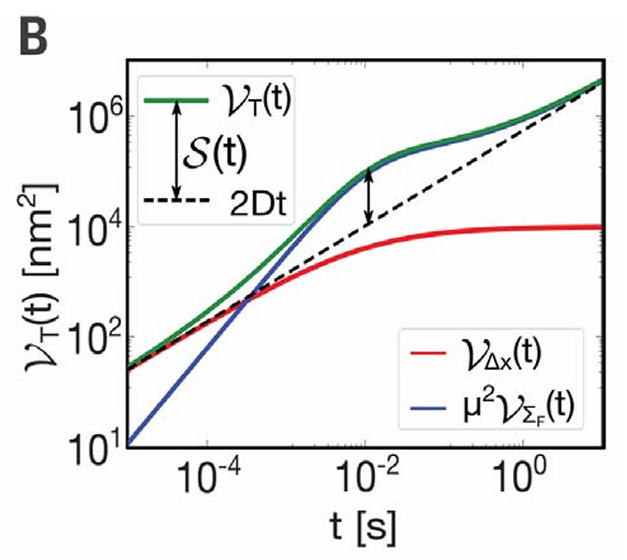
\includegraphics[width=5cm]{vsr_fig1b.png}  
  \end{center}
  \caption{VSR をNESSに適用した場合のグラフ}
\end{figure}

\newpage 
今,導出した VSR とエントロピー生成率 $\sigma$を結びつける.
今考えているLangevin方程式において熱はつぎのように定義される.
\begin{equation}
  d \hat{Q} := - \frac{\partial U}{\partial x} \circ  d \hat{x} 
\end{equation}
ただし $\hat{\cdot}$ のように,確率変数についてはハットをつける.また,$\circ $は Stratonovich 積を表す.
今は,$F$を$- \frac{\partial U}{\partial x}$と仮定しているため,エントロピー生成は
\begin{equation}
  \label{entropyprob1}
  \sigma dt = \frac{1}{k_B T} \langle F(t) \circ dx(t) \rangle
\end{equation}
となる.Stratonovich 積の定義より
\begin{align}
  \langle F(t) \circ dx(t) \rangle &= \frac{1}{2} \langle \qty{ F(t + dt) + F(t) } \qty{ x(t + dt) - x(t) } \rangle \\
  &= \frac{1}{2} \langle \qty{ F(t + dt) + F(t) } \qty{ y(t + dt) - y(t) + vdt } \rangle \quad (y(t) = x(t) - vt)
\end{align}
となる.ただし,$v$ は粒子の平均速度である.
ここでつぎの量を考える.
\begin{equation}
  C_{yF}(dt) - C_{Fy} (dt) = \langle y(dt)F(0) \rangle - \langle y(0)F(dt) \rangle
\end{equation}
相関関数なので
\begin{equation}
  C_{yF}(dt) - C_{Fy} (dt) = \langle y(t + dt)F(dt) \rangle - \langle y(dt)F(t + dt) \rangle
\end{equation}
にも注意しておく.そうすれば,$\langle F(t) \circ dx(t) \rangle$は
\begin{align}
  \langle F(t) \circ dx(t) \rangle &= \frac{1}{2} \langle \qty{ F(t + dt)y(t + dt) - F(t)y(t)} + \qty{ F(t + dt)vdt + F(t)vdt} + \qty{ F(t)y(t + dt) - F(t + dt)y(t) } \rangle \\
  &= \frac{1}{2} \qty[ C_{yF}(dt) - C_{Fy} (dt) ] + \frac{1}{2} \cdot 2 \langle F(t) \rangle vdt \\
  &= \frac{1}{2} \qty[ C_{yF}(dt) - C_{Fy} (dt) ] + \frac{v^2}{\mu } dt \quad \quad (\because \langle F(t) \rangle = \frac{v}{\mu })
\end{align}
となる.ここで,$\ave{F(t)}, \ave{y(t)}, \ave{F(t)y(t)}$ は時間に依存しないことを用いた.
これをTaylor展開する.
\begin{align}
  \langle F(t) \circ dx(t) \rangle &= \frac{1}{2} \qty[ \qty( C_{yF}(0) + \dot{C}_{yF}dt + \cdots ) - \qty( C_{Fy}(0) + \dot{C}_{Fy}dt + \cdots  ) ] + \frac{v^2}{\mu } dt \\
  &= \frac{1}{2} \qty[ \dot{C}_{yF} - \dot{C}_{Fy} ] dt + \frac{v^2}{\mu } dt
\end{align}
$D=k_B T \mu$に注意して,式(\ref{entropyprob1})に戻せば
\begin{equation}
  \label{s15}
  \sigma|_{t = 0} = \frac{1}{2k_B T} \qty[ \dot{C}_{yF} - \dot{C}_{Fy} ] + \frac{v^2}{D}
\end{equation}
となり,$\mathcal{S} (t) $を用いて書くと
\begin{equation}
  \label{vsr3}
  \sigma = \frac{1}{4D} \frac{\partial^2}{\partial t^2} \mathcal{S} (t) |_{t = 0}  + \frac{v^2}{D}
\end{equation}
となる.この $\sigma$ の表式は理論から直接導かれたものであり,実験的に求められる $\sigma$ と区別する必要がある場合は,特に $\sigma_{th}$ と書くことにする.\\
\quad 続いて実験的に $\sigma$を求めるための表式を導く.式(\ref{vsr1}) の両辺を $D( =k_B T \mu )$ で割る.
\begin{equation}
  \mathcal{V} _{\Delta x} (t) + \mu^2 \mathcal{V} _{\Sigma_F} (t) = 2Dt + 2\mu \int_0^t ds ( C_{xF} (s) - C_{Fx} (s) )
\end{equation}
\begin{equation}
  \therefore \quad \frac{1}{k_B T} \qty( \frac{1}{\mu} \mathcal{V} _{\Delta x} (t) + \mu \mathcal{V} _{\Sigma_F} (t)) = 2t + \frac{2}{k_B T} \int_0^t ds ( C_{xF} (s) - C_{Fx} (s) )
\end{equation}
両辺を2回微分して,$t=0$を考える.
\begin{equation}
  \frac{1}{k_B T} \qty( \frac{1}{\mu} \frac{\partial^2}{\partial t^2} \mathcal{V} _{\Delta x} (t) + \mu \frac{\partial^2}{\partial t^2} \mathcal{V} _{\Sigma_F} (t)) = \frac{2}{k_B T} ( \dot{C}_{xF} (t) - \dot{C}_{Fx} (t) ) \quad \text{for \ t = 0}
\end{equation}
ここで\footnote{この関係は,定義を微分すれば求まる}
\begin{equation}
  \frac{\partial^2}{\partial t^2} \mathcal{V} _{\Sigma_F} (t)|_{t = 0} = 2 \mathcal{V}_F (0)
\end{equation}
と,式 (\ref{s15}) を用いて 
\begin{equation}
  \sigma = \frac{v^2}{D} + \frac{1}{k_B T} \qty( \frac{1}{4 \mu } \frac{\partial^2}{\partial t^2} \mathcal{V} _{\Delta x} (t)|_{t = 0} + \frac{\mu }{2} \mathcal{V}_F (0) )
\end{equation}
これによって分散から $\sigma$ を求めることができる.これを$\sigma_{th}$ と区別する必要があるときは,$\sigma_{exp}$とかく.
以上で導いた VSR を簡単な NESS に適用してみる.\\
\quad 以上で2つの $\sigma$ が出た.これらを注意して区別する必要があるため,それらの強調のためにも再度示しておく.
\begin{tcolorbox}
  \begin{equation}
    \label{sigma_th}
    \sigma_{th} = \frac{1}{4D} \frac{\partial^2}{\partial t^2} \mathcal{S} (t) |_{t = 0}  + \frac{v^2}{D}
  \end{equation}
  \begin{equation}
    \label{sigma_exp}
    \sigma_{exp} = \frac{v^2}{D} + \frac{1}{k_B T} \qty( \frac{1}{4 \mu } \frac{\partial^2}{\partial t^2} \mathcal{V} _{\Delta x} (t)|_{t = 0} + \frac{\mu }{2} \mathcal{V}_F (0) )
  \end{equation}
\end{tcolorbox}

\newpage 
\section{方法}
コロイド粒子を用いた実験は,文献[22] に記載されている光ピンセットで行った.
赤血球(RBC)は,健康なドナーの指先から採取した.
リン酸緩衝食塩水(PBS)溶液には,130 mMのNaCl,20 mMの K/Na リン酸緩衝液,10 mMのグルコース,そして1 mLあたり1 mgのウシ血清アルブミンが含まれる.
光ピンセット(OT)を用いた伸展実験では,4 mLの血液を1 mLのPBSで希釈した.
RBCはOTセンシングのためにビオチン化した(文献[11]を参照せよ).
光学顕微鏡(OM)測定のために,遠心分離(5000 g for 10 min in 4℃)後に得られたRBCペレットは,PBS溶液で 1:15 に懸濁した(文献[23]を参照せよ).
OT実験における接触面積は,画像のガウスピラミッド表現に基づいたマルチスケール特徴抽出器を用いて推定し,その後ラプラシアン再構築を行った.
OTセンシングには,文献[11]からの推定値を使用した.

\newpage 
\section{水中で牽引したコロイド粒子}
光ピンセットにより水中で牽引される(速度 $v$ )コロイド粒子を考える.
この系の運動は解析的でVSRの正当性が確認できる.なお,摩擦係数 $\gamma $は
\begin{equation}
  \gamma = \frac{1}{\mu }
\end{equation}
であり,速度 $v$で牽引する光ピンセットによるポテンシャルは
\begin{equation}
  U(x, t) = \frac{k}{2} (x -vt)
\end{equation}
である.この系におけるエントロピー生成を推定する.まずは理論的に予測する.\\
\quad 簡単のために,$y(t) = x(t) - vt$ として $y(t)$ で考える.
先と同じLangevin方程式に,$y(t) = x(t) -vt$ と $F(t) = k(vt - x)$ を代入して,
\begin{equation}
  \dot{x} (t) = \mu F(t) + \sqrt{2D} \eta (t)
\end{equation}
\begin{equation}
  \dot{y}(t) + v = \mu k (vt - y(t) - vt) + \sqrt{2D} \eta(t)
\end{equation}
$\mu = \gamma^{-1}$ を使って整理すると
\begin{equation}
  \label{s21}
  \gamma \dot{y} (t) = -k y(t) - \gamma v + \sqrt{2 k_B T \gamma } \eta(t)
\end{equation}
となる.\\
\quad $y(t) = x(t) -vt$ であることより,$y(t)$ と$x(t)$には定数のずれしかないので
\begin{equation}
  \mathcal{V}_{\Delta x} (t) = \mathcal{V}_{\Delta y} (t)
\end{equation}
である.ここで式 (\ref{s21}) の微分方程式より $\mathcal{V}_{\Delta y} (t)$ を求める.少し変形すると
\begin{equation}
  \dot{y} (t) = - \frac{1}{\tau_r} y(t) - v + \sqrt{\frac{2 k_B T}{\gamma}} \eta(t)
\end{equation}
となる.ただし,$\tau_r = \frac{\gamma}{k}$ である.ここで,$y(t)$ を定数分だけずらしても,$\dot{y}(t)$ には影響がないことに注意すると,これから $\mathcal{V}_{\Delta y} (t)$ を求める上では,$v$ の項は考える必要はないことになる.
したがって考えるべき微分方程式は
\begin{equation}
  \dot{y} (t) = - \frac{1}{\tau_r} y(t) + \sqrt{\frac{2 k_B T}{\gamma}} \eta(t)
\end{equation}
である.この微分方程式の解はを形式的に解くと,つぎのような表現が得られる.
\begin{equation}
  y(t) = \exp( -\frac{t}{\tau_r}) y(0) + \sqrt{\frac{2k_B T}{\gamma}} \int_0^t \exp( -\frac{1}{\tau_r} (t-s) ) \eta(s) ds 
\end{equation}
また,$\mathcal{V}_{\Delta y} (t)$というのは,今の場合は
\begin{align}
  \mathcal{V}_{\Delta y} (t) &= \ave{(\Delta y (t))^2} - 0 \\
  &= \ave{(y(t) - y(0))^2} \\
  &= \ave{(y(t))^2} 
\end{align}
である.そうすれば,先ほどの解の2乗を考え,時間平均をとることで分散が求まる.
\begin{align}
  \ave{(y(t))^2}  &= \frac{2k_B T}{\gamma} \int_0^t \int_0^t ds ds' \exp( -\frac{1}{\tau_r} (2t-s-s') ) \ave{\eta(s) \eta(s') } \\
  &= \frac{2k_B T}{\gamma} \int_0^t \int_0^t ds ds' \exp( -\frac{1}{\tau_r} (2t-s-s') ) \delta(s-s') \\
  &= \frac{2k_B T}{\gamma} \int_0^t ds \exp( -\frac{2}{\tau_r} (t-s) ) \\
  &= \frac{2k_B T}{\gamma} \exp( -\frac{2t}{\tau_r} ) \int_0^t ds \exp( \frac{2s}{\tau_r} ) \\
  &= \frac{2k_B T}{\gamma} \exp( -\frac{2t}{\tau_r} ) \frac{\tau_r}{2} \qty(\exp(\frac{2t}{\tau_r}) - 1) \\
  &= \frac{k_B T}{k} \qty(1 - \exp(-\frac{2t}{\tau_r})) \\
\end{align}
しかし,論文では下のような解になっていた.
\begin{equation}
  \mathcal{V}_{\Delta y} (t) = \frac{2 k_B T}{k} \qty( 1 - e^{-\frac{t}{\tau_r}} )
\end{equation}
以下,論文に合わせるために,この解を用いる.\\
\quad これを用いて,
\begin{equation}
  \mathcal{V}_{\Sigma F} (t) = 2 k_B T \gamma \qty( t - \tau_r \qty( 1 - e^{-\frac{t}{\tau_r}} ) )
\end{equation}
も計算できる.以上の結果を用いて
\begin{equation}
  \mathcal{V}_{\Delta x} (t) + \mu^2 \mathcal{V}_{\Sigma F} (t) = 2Dt 
\end{equation}
が成り立ち,
\begin{equation}
  \mathcal{S} (t) = 0 
\end{equation}
と分かり,エントロピー生成は
\begin{equation}
  \sigma_{th} = \gamma v^2
\end{equation}
と計算できる.ここで式 (\ref{sigma_th}) を用いた.\footnote{
$\mathcal{S} (t) = 0 $ と $\sigma = \gamma v^2$ は調和ポテンシャルに限らず,任意の時間に依存するポテンシャル $U(x - vt)$ に対して成り立つ.
この下で,Reversed thermosynamic uncertainly relation が成り立つ.
$\mathcal{S} (t) = 0 $であるとき,式 (\ref{vsr2})から,
\begin{equation}
  \mathcal{V}_{\Delta x} (t) \leqslant 2Dt 
\end{equation}
\begin{equation}
  \mathcal{V}_{\Sigma F} (t) \leqslant \frac{2D}{\mu ^2} t 
\end{equation}
が分かる.もちろん $\mathcal{S} (t) \neq  0 $ のときは,成り立たない.\\
\quad ここで光ピンセットからビーズに行う仕事
\begin{equation}
  W(t) = v \Sigma _F (t) = v \int_0^t ds F(s)
\end{equation}
の分散 $\mathcal{V}_{W} (t)$ を用いて,不等式を書き直すことを考える.すぐ上の定義より
\begin{equation}
  \mathcal{V}_{W} (t) = v \mathcal{V}_{\Sigma F} (t)
\end{equation}
なので,
\begin{equation}
  \frac{\mathcal{V}_{W} (t)}{v^2} \leqslant \frac{2D}{\mu^2} t 
\end{equation}
\begin{equation}
  \frac{\mathcal{V}_{W} (t)}{v^2 \gamma^2} \leqslant 2Dt 
\end{equation}
さらに,
\begin{equation}
  \langle W(t) \rangle = \gamma v^2 t = \sigma t 
\end{equation}
を用いて
\begin{equation}
  \frac{\mathcal{V}_{W} (t)}{v^2 \gamma^2} \leqslant 2Dt  = 2 k_B T t \frac{1}{\gamma}
\end{equation}
\begin{equation}
  \therefore \quad \frac{\sigma }{k_B T} \leqslant \frac{2 \langle W(t) \rangle^2}{t \mathcal{V}_{W} (t)}
\end{equation}
と書き直せる.これが Reversed thermosynamic uncertainly relation である.} \\
\quad 続いて系のエントロピー生成を実験的にも確認する.それが図3である.

\begin{figure}[H]
  \begin{center}  
  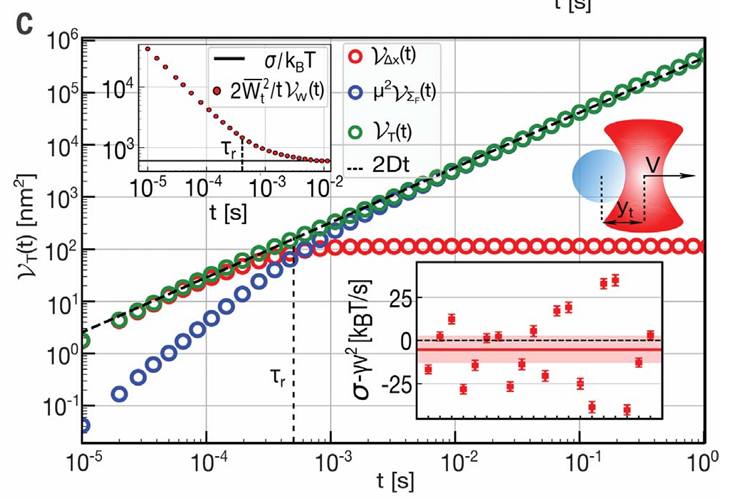
\includegraphics[width=15cm]{vsr_fig1c.png}  
  \end{center}
  \caption{水中で牽引したコロイド粒子}
\end{figure}

まずは右下のグラフからみる.この縦軸は式 (\ref{sigma_exp}) より
\begin{equation}
  \sigma_{exp} = \frac{v^2}{D} + \frac{1}{k_B T} \qty( \frac{1}{4 \mu } \frac{\partial^2}{\partial t^2} \mathcal{V} _{\Delta x} (t)|_{t = 0} + \frac{\mu }{2} \mathcal{V}_F (0) )
\end{equation}
\begin{equation}
  \therefore \quad \sigma_{exp} - \gamma v^2 = \frac{1}{4 \mu } \frac{\partial^2}{\partial t^2} \mathcal{V} _{\Delta x} (t)|_{t = 0} + \frac{\mu }{2} \mathcal{V}_F (0) \quad (\because \quad D = \frac{\gamma }{k_B T})
\end{equation}
となり,この右辺を実験で測定している.その結果が右下のグラフであり,$\sigma = 0$ が分かり,これは理論的な予測 $\sigma_{th}$ と一致する.\\
\quad 左上のグラフは注釈で説明した Reversed thermosynamic uncertainly relation の確認である.十分大きな $t$ に対して,不等関係が厳しくなっていることが分かる.\\
\quad 中央のグラフでは,式 (\ref{vsr2}) より
\begin{equation}
  \mathcal{V} _{\Delta x} (t) + \mu^2 \mathcal{V} _{\Sigma_F} (t) = 2Dt + \mathcal{S} (t)
\end{equation}
$\mathcal{S} (t) = 0$ を確認している.

\newpage 
\section{The stochastic switching trap}
The stochastic switching trap (SST) モデルに対して,VSR を適用してみる.
このモデルでは光トラップされた粒子にアクティブ力が加えられ,トラップ位置 $\lambda (t)$ が $( \lambda_+, \lambda_- )$ という2つの値 ($\Delta \lambda := \lambda_+ - \lambda_-$) でランダムにスイッチする(下図).

\begin{figure}[H]
  \begin{center}  
  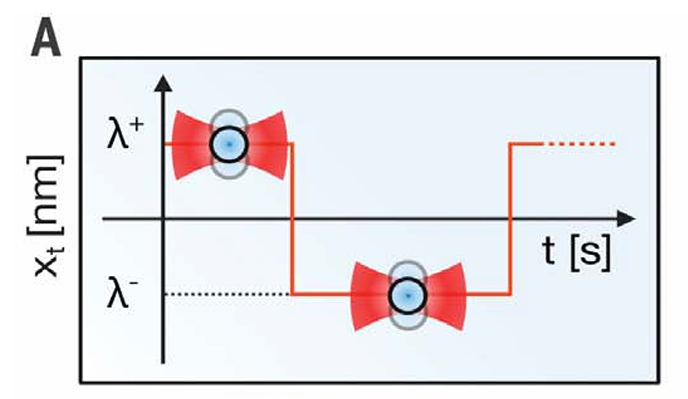
\includegraphics[width=5cm]{vsr_fig2a.png}  
  \end{center}
  \caption{SST model}
\end{figure}

スイッチは,それぞれの位置において $w_+, w_-$ の割合で起こる.
また,これらの比率は
\begin{equation}
  \frac{w_-}{w_+} = \frac{q}{1-q}
\end{equation}
というように,$\lambda_+$ に存在する確率 $q$ で表すことにする.\\
\quad ここから $\sigma$ を求める.
光トラップのポテンシャルは
\begin{equation}
  U(x(t), \theta(t)) = k \frac{(x(t) - \theta(t) \Delta \lambda)^2}{2}
\end{equation}
で,$\theta (t)$ は $\theta (t) = {0, 1}$ の確率変数である.$w_-$ は $\lambda_- \to \lambda_+$ に遷移する割合で,$w_+$ はその逆である.便利のために $w = w_+ + w_-$ という文字を導入しておく.
$\theta (t)$ の時間平均は $q$ に対応し,
\begin{equation}
  q = \ave{\theta(t)} = \frac{w_-}{w}
\end{equation}
である.簡単のために $\lambda_- = 0, \lambda_+ = \Delta \lambda$ とする.\\
\quad この下で EOM は
\begin{equation}
  \dot{x} (t) = - \mu k (x(t) - \Delta \lambda \theta (t)) + \sqrt{2 k_B T \mu} \eta(t)
\end{equation}
となって,今考えているNESSでは $\ave{\dot{x}(t)} = 0$ である.したがって,$\ave{x(t)} = q \Delta \lambda$ である.
前節でも導入した $\tau_r$ を考え,その逆数を $w_r$ をする.
\begin{equation}
  w_r = \frac{1}{\tau_r} = \mu k
\end{equation}
\quad 以上の設定で $\mathcal{V} _{\Delta x} (t), \mathcal{V} _{\Sigma_F} (t)$ を計算する.
それらより,$\mathcal{S} (t)$ の表式が求まり,$\sigma $も求まる.\\
\quad $\mathcal{V} _{\Delta x} (t), \mathcal{V} _{\Sigma_F} (t)$ の計算の詳細は sup.mat に書いてある.(書き込むのが間に合いませんでした)
\footnote{
計算の概略をメモする.
まずはEOMを時間幅 $dt$ で離散化する.すなわち
\begin{equation}
  x(t+dt) = x(t) - w_r x(t) dt + \mu k \Delta \lambda \theta (t)dt + \sqrt{ 2 k_B T \mu  } d B^x(t)
\end{equation}
\begin{equation}
  \theta(t+dt) = \theta(t) + (1 -2\theta(t)) \Theta(w_{\theta(t)}dt-r)
\end{equation}
であって,ここで$dB^x(t)$ はウィーナー過程に従う変数,$\Theta$はヘビサイド関数である.
これらに $x_0$ または $\theta(0)$ をかけて統計平均をとることで,4本の式を得る.
ここでは1本だけ書く.
\begin{equation}
  \pdv{C_{xx}}{t} (t) = - w_r C_{xx}(t) + \mu k \Delta \lambda C_{\theta x} (t)
\end{equation}
さらに,離散化したEOMを変形することで,$t=0$ の初期条件を4本得る.これも1つだけメモ.
\begin{equation}
  C_{xx} (0) = \Delta \lambda^2 q^2 + \frac{k_B T}{k} + \frac{k \Delta \lambda^2 q(1-q)\mu }{(w+w_r)}
\end{equation}
以上4式より,相関関数の具体的な表式を求める.例えば $C_{xx}(t)$ は 
\begin{equation}
  C_{xx} (t) = \Delta \lambda^2 q^2 + \qty( \frac{k_B T}{k} + \frac{k \Delta \lambda^2 q(1-q)\mu }{(w + w_r)} ) \exp(- w_r t) + \cdots
\end{equation}
これが $C_{x \theta}, C_{\theta \theta}, C_{\theta x}$ についても求まる.
ここで 
\begin{equation}
  \mathcal{V}_{\delta x} (t) = 2 (C_{xx}(0) - C_{xx}(t))
\end{equation}
より $\mathcal{V}_{\delta x} (t) $ が求まり,
\begin{equation}
  \mathcal{V}_{\Sigma_F} (t) = \int_0^t dt' \int_0^t dt'' \ave{F(t')F(t'')} = 2 \int_0^t dt' \int_0^t dt'' \ave{F(t'')F(0)}
\end{equation}
より,$\mathcal{V}_{\Sigma_F} (t)$が求まる.これら分散より,$\mathcal{S}(t)$ が分かり,$\sigma$も求まる.

}

ここでは結果のみ記すと,
\begin{equation}
  \mathcal{V} _{\Delta x} (t) = 2 \qty[ \qty(\frac{k_B T}{k} + \frac{\epsilon^2 \mu}{k (w + w_r)}) \qty(1 - \exp(- w_r t)) + \frac{\epsilon^2 \mu^2}{w^2 - w_r^2} \qty( \exp(-wt) - \exp(-w_r t) ) ]
\end{equation}
\begin{equation}
  \mathcal{V} _{\Sigma_F} (t) = \frac{2k_B T t}{\mu} + \frac{2k_B T}{\mu^2 k} \qty( 1 - \exp(-w_r t) ) + \frac{2\epsilon^2}{w_r (w + w_r)} \qty( 1 - \frac{w \exp(-w_r t)}{w - w_r} + \frac{w_r \exp(-w t)}{w - w_r})
\end{equation}
となる.ただし, $\epsilon = k \Delta \lambda \sqrt{ q (1-q) }$ である.これらを用いて,
\begin{equation}
  \mathcal{S} (t) = \frac{4 \epsilon^2}{k (w + w_r)} \qty( 1 - \frac{w \exp(-w_r t)}{w - w_r} + \frac{w_r \exp(-w t)}{w - w_r})
\end{equation}
と計算できる.そうして
式 (\ref{vsr3}) より 
\begin{equation}
  \sigma_{th} = \epsilon^2 \mu \frac{w}{w + w_r}
\end{equation}
と,$\sigma$ が求まる.\\
\quad 実験結果を見る.次の図は $\mathcal{V}_T (t) =  \mathcal{V} _{\Delta x} (t) + \mu^2 \mathcal{V} _{\Sigma_F} (t)$ の時間変化を3つの$\Delta \lambda$に対して調べたものであり,図の右下に挿入された図は,$\mathcal{V}_T (t)$の2つの項の寄与を示したものである.

\begin{figure}[H]
  \begin{center}  
  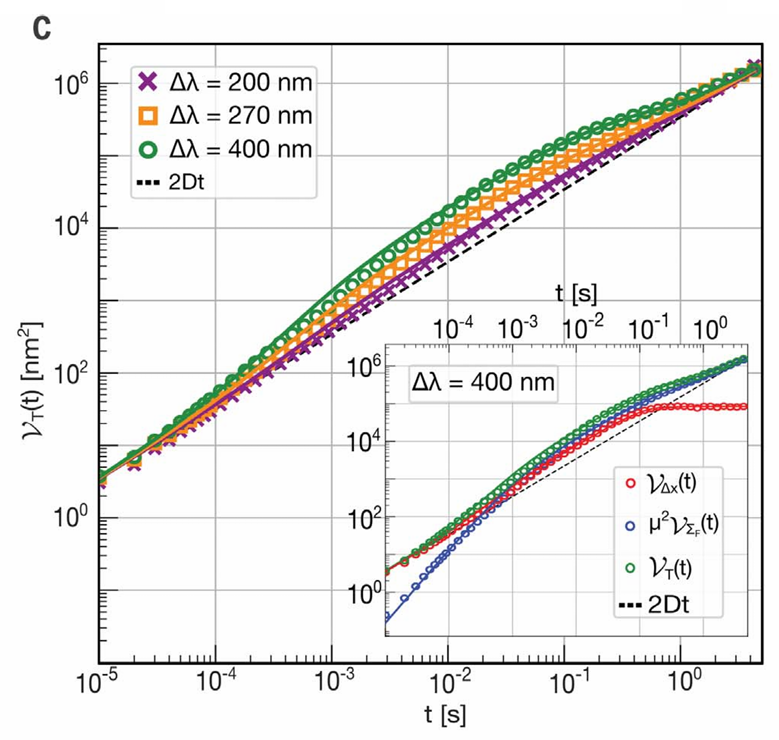
\includegraphics[width=10cm]{vsr_fig2c.png}  
  \end{center}
  \caption{SST model の結果}
\end{figure}

十分長い時間が経てば,$\mathcal{V}_T (t)$ が $2Dt $に収束することが分かる.\\
\quad 次の図は$\Delta \lambda = 280 nm$ における $\sigma_{th}$ と $\sigma_{exp}$ の比較である.

\begin{figure}[H]
  \begin{center}  
  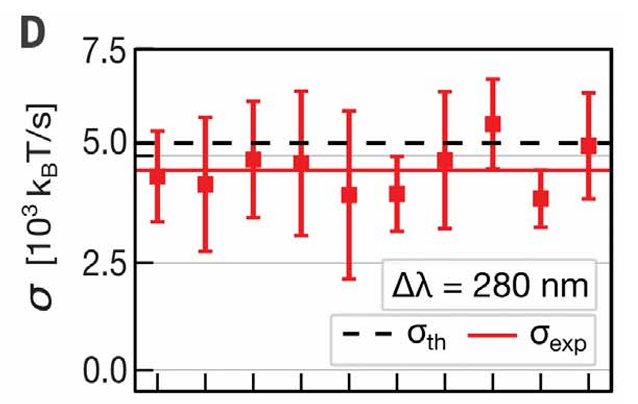
\includegraphics[width=5cm]{vsr_fig2d.png}  
  \end{center}
  \caption{$\Delta \lambda = 280 nm$ における $\sigma_{th}$ と $\sigma_{exp}$ の比較}
\end{figure}

次の図は,$\Delta \lambda $を変化させた場合の比較である.

\begin{figure}[H]
  \begin{center}  
  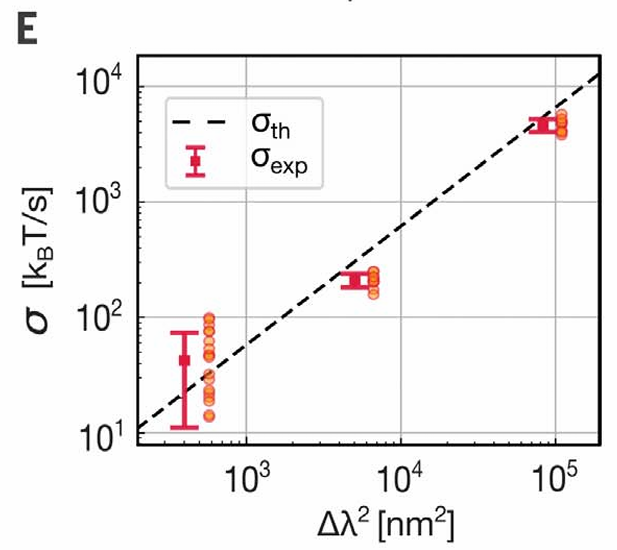
\includegraphics[width=5cm]{vsr_fig2e.png}  
  \end{center}
  \caption{$\Delta \lambda $を変化させた場合の比較}
\end{figure}

いずれの場合も良い一致をみせている.\\
\quad ここからメモです.\\
\quad $w_{\theta (t)}$ は $\theta (t)$ に依存する jumping rate,$r$ は$[0,1]$の一様分布に従う確率変数.\\
\quad $\Theta (\cdot)$ の引数が正になるとき,jumping が起こる.
逆に$\Theta (\cdot)$ の引数が負になるとき,その状態を保つ.\\
相関関数の初期条件 ($C_{\theta \theta} (0)$など)を求めるときは,$dt$の次数のものに注目すればよい.例えば
\begin{equation}
  \ave{\theta(t+dt)\theta(0)} - \ave{\theta(t)\theta(0)} = w_- q dt - w \ave{\theta(t)\theta(0)}dt 
\end{equation}
は左辺をテイラー展開して,
\begin{equation}
  \frac{\partial}{\partial t} \ave{\theta(t)\theta(0)} dt = w_- q dt - w \ave{\theta(t)\theta(0)}dt
\end{equation}
より 
\begin{equation}
  \frac{\partial}{\partial t} \ave{\theta(t)\theta(0)} = w_- q - w \ave{\theta(t)\theta(0)}  
\end{equation}
これを $t = 0$にして 
\begin{equation}
  \frac{\partial}{\partial t} \ave{\theta(0)\theta(0)} = w_- q - w \ave{\theta(0)\theta(0)}
\end{equation}
相関関数は $t$ に依存しないので,
\begin{equation}
  \ave{\theta(0)\theta(0)} = q^2
\end{equation}
となる.\footnote{これは論文と次数が異なるが,論文の他の式を見ても $q^2$ が正しいと考えた.}\\
\quad 他の初期条件については,謎の項がついていたりしてよく分からない.\\
\quad 微分方程式を出すときに,$C_{xx}, C_{x \theta}$ の方は良いのだが,$C_{\theta x}, C_{\theta \theta}$ の方でヘビサイド関数をどのように処理しているのか分からない.
\begin{equation}
  \theta (t+dt) = \theta (t) + (1 -2 \theta(t)) \Theta_H (w_{\theta(t)}dt - r) 
\end{equation}
に $\theta (0)$ をかけて,アンサンブル平均をとると,
\begin{equation}
  C_{\theta \theta} (t+dt) - C_{\theta \theta }(t) = \ave{ \theta (0) \Theta_H (w_{\theta(t)}dt - r)} - 2\ave{ \theta (t) \theta(0) \Theta_H (w_{\theta(t)}dt - r)}
\end{equation}
左辺は $dt$ で割って,$\partial_t C_{\theta \theta} (t)$ になるのだと思うが,右辺はどのように処理できるのか分からない.
論文で示されている式より,つぎのような関係があることが推測できる.
\begin{equation}
  \ave{ \theta (0) \Theta_H (w_{\theta(t)}dt - r)} = w_- q dt 
\end{equation}
\begin{equation}
  \ave{ \theta (t) \theta(0) \Theta_H (w_{\theta(t)}dt - r)} = \frac{1}{2} w C_{\theta \theta}(t) dt
\end{equation}
$\Theta (\cdot)$ の引数が正になるとき,jumping が起こることを思い出せば,感覚的には正しそうな式になっている.

\newpage 
\section{Reduced VSR}
これまでは $F^I (t) = 0$ である場合を考え,測定できない自由度については心配する必要がなかった.
しかし,見えない自由度がある場合であっても,Reduced VSR を用いることで,$x(t)$ のみの情報から解析することができる.
実際には測定することのできない力 $F^I (t)$ は,測定できる変数 $x(t)$に依存しないことと,$F^I (t)$の時間相関を知っていなければ解析することはできないことには注意が必要である.\\
\quad $F^M (t) = -kx(t)$ である場合は,つぎのような Reduced VSR が成り立つ.
\begin{equation}
  \mathcal{V} _{\Delta x} (t) + \mu^2 k^2 \mathcal{V} _{\Sigma_x} (t) = 2Dt + \tilde{\mathcal{S}}(t)
\end{equation}
ただし,$\mathcal{V} _{\Sigma_x} (t) = \int_0^t ds x(s)$ である.また,$\sigma $ は先に示した方法では求まらず,$\tilde{\mathcal{S}}(t)$ は $\mathcal{S} (t)$と異なることに注意が必要である.\\
\quad 実際に $\sigma $を求めるときの手順は次の通りである.この方法は,$F^I$ が線形である場合は適用することができる.
\begin{enumerate}
  \item 設定したモデルに対して $S(t)$ と $\tilde{\mathcal{S}}(t)$ の解析的な解を求める
  \item 式 (\ref{vsr3}) を用いて理論的な $\sigma$を求める.これを $\sigma_{th}$ とする.
  \item モデルから得られた$\tilde{\mathcal{S}}(t)$を用いて,Reduced VSR を実験データに対してフィッティングし,モデルのパラメータを決定する.
  \item 求められたモデルのパラメータを $\sigma_{th}$ に代入して,$\sigma$を求める.
\end{enumerate}
\quad 以上の方法を適用した例を見る前に,Reduced VSR を導出する.ここでは,プローブ粒子に対して線形な力 $-kx(t) $ と,測定できない力 $F^I (t)$がかかっている場合を考える.
すなわち,$F(t) = -kx(t) + F^I (t)$ とした Langevin 方程式を考える.
\begin{equation}
  \dot{x} (t) + k \mu x(t) = \mu F^I (t) + \sqrt{2D} \eta (t)
\end{equation}
ここからの基本的な処理は VSR を求めたときと同様の方法である. \\
\quad まずは $0 \to t$ で積分し,見やすさのため文字で置き換える.
\begin{equation}
  \Delta x(t) + k \mu \int_0^t x(s) ds = \mu \int_0^t F^I (s) ds + \sqrt{2D} \int_0^t \eta(s) ds 
\end{equation}
\begin{equation}
  \Delta x(t) + k \mu \Sigma_x (t) = \mu \Sigma_{F^I} (t) + \sqrt{2D} \int_0^t \eta(s) ds 
\end{equation}
両辺を2乗して,
\begin{equation}
  \label{totyu4}
  \qty{\Delta x(t)}^2 + 2 \qty{\Delta x(t)} \mu k \Sigma_x (t) + k^2 \mu^2 \qty{\Sigma_x (t)}^2 = \mu^2 \qty{\Sigma_{F^I} (t) }^2 + 2D \int_0^t ds \int_0^t ds' \eta(s) \eta(s') + 2 \sqrt{2D} \mu \Sigma_{F^I} (t) \int_0^t \eta (s) ds 
\end{equation}
ここからの変形のために,いくつかの量について計算しておく.
\begin{equation}
  \label{totyu5}
  \langle \qty{\Delta x(t)}^2 \rangle = \mathcal{V} _{\Delta x} (t) + \langle \Delta x(t) \rangle ^2 = \mathcal{V} _{\Delta x} (t)
\end{equation}
\begin{equation}
  \langle \qty{\Sigma_x (t)}^2 \rangle = \mathcal{V} _{\Sigma_x} (t) + \langle \Sigma_x (t) \rangle ^2 {=} \mathcal{V} _{\Sigma_x} (t) 
\end{equation}
\begin{equation}
  2D \int_0^t ds \int_0^t ds' \eta(s) \eta(s') = 2Dt 
\end{equation}
\begin{equation}
  C_{F^I F^I} (u) := \langle F^I (u) F^I (0) \rangle - \langle F^I (0) F^I (0) \rangle = \langle F^I (u) F^I (0) \rangle
\end{equation}
\begin{equation}
  \label{int1}
  \int_0^t ds \int_0^t du \langle F(s) F(u) \rangle = 2 \int_0^t ds \int_0^s du \langle F(y) F(0) \rangle
\end{equation}
\begin{equation}
  \label{totyu3}
  \qty{\Delta x(t)} \mu k \Sigma_x (t) = 0
\end{equation}
式 (\ref{int1}) については,つぎのような変形を考えればよい.
\begin{align}
  (\text{左辺}) &= \int_0^t ds \int_0^t du \langle F(s-u) F(0) \rangle \quad (\because \text{相関関数は時刻をずらせる}) \\
  &= \int_0^t ds \int_s^{s-t} (-dy) \langle F(y) F(0) \rangle \quad (y = s - u) \\
  &= \int_0^t ds \int_{s-t}^s dy \langle F(y) F(0) \rangle \\
  &= 2 \int_0^t ds \int_0^s dy \langle F(y) F(0) \rangle \quad (\text{下図を参考にせよ.})
\end{align}
ただし, $y = 0$より上の領域と,下の領域で相関関数が同じ振る舞いをすることは自明ではない.

\begin{figure}[H]
  \begin{center}  
  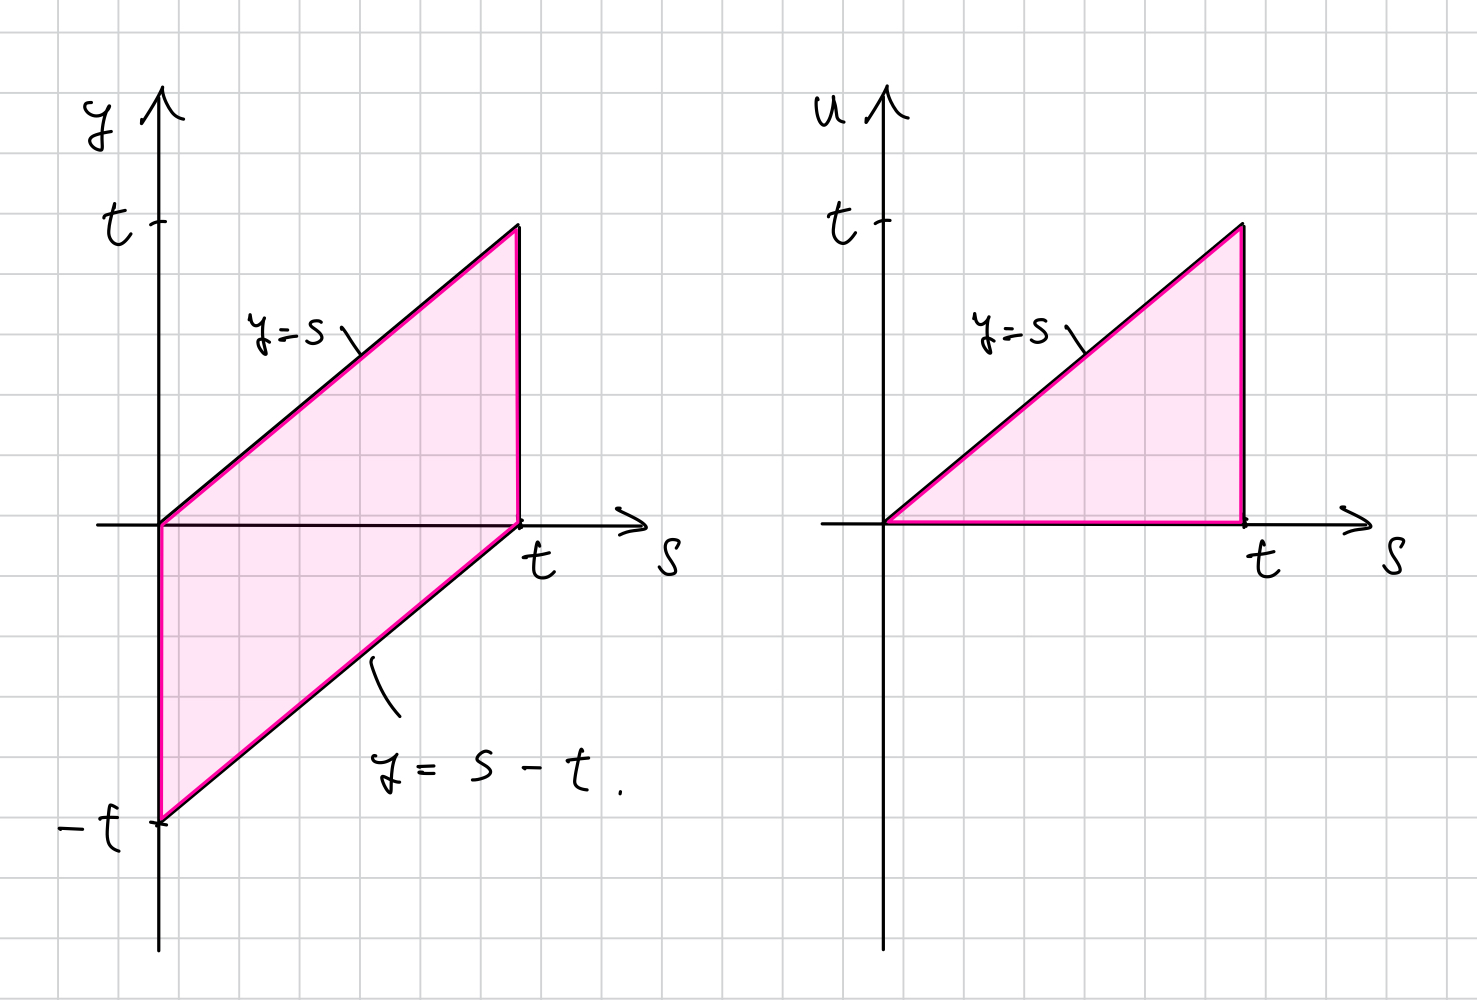
\includegraphics[width=7cm]{int_inv.jpg}  
  \end{center}
  \caption{式 (\ref{int1}) の変形にて参考にする図}
\end{figure}

式 (\ref{totyu3}) については,次の変形をみよ.
\begin{align}
  \Delta x(t) \Sigma_x (t) &=   \Delta x(t) \int_0^t x(s) ds \\
  &= \int_0^t x(t)x(0) ds - \int_0^t x(0) x(s) ds 
\end{align}
であって,
\begin{align}
  \int_0^t x(0) x(s) ds &= \int_t^0 x(0)x(t-s') ds' \quad (s' = t-s) \\
  &= \int_0^t x(0) x(t-s') ds' \\
  &= \int_0^t x(s') x(t) ds'
\end{align}
となるため,
\begin{equation}
  \Delta x(t) \Sigma_x (t) = \int_0^t x(t)x(0) ds - \int_0^t x(0) x(s) ds = 0
\end{equation}
である.\\
\quad 式 (\ref{totyu4}) に,式 (\ref{totyu5}) から 式 (\ref{totyu3}) を代入することで,次を得る.
\begin{equation}
  \mathcal{V} _{\Delta x} (t) + \mu^2 k^2 \mathcal{V} _{\Sigma_x} (t) = 2Dt + 2\mu^2 \int_0^t ds \int_0^s du C_{F^I F^I} (u) + 4\mu \sqrt{2D} \int_0^t ds \int_0^s du C_{F^I \eta } (u)
\end{equation}
これは論文と,右辺の最後の項がずれている.論文では,
\begin{equation}
  \mathcal{V} _{\Delta x} (t) + \mu^2 k^2 \mathcal{V} _{\Sigma_x} (t) = 2Dt + 2\mu^2 \int_0^t ds \int_0^s du C_{F^I F^I} (u) + 2\mu \sqrt{2D} \int_0^t ds \int_0^s du C_{F^I \eta } (u)   
\end{equation}
となっている.ところで,$\tilde{\mathcal{S}}(t)$ をつぎのように定義すると便利である.\footnote{より一般には,つぎのように書ける.
\begin{equation}
  \tilde{\mathcal{S}}(t) = 2 \mu \int_0^t ds \int_0^s du \qty( \mu k C_{F^I x}(u) - \dot{C}_{F^I x} (u) )
\end{equation}
この表式は後ほどRBC modelで用いる.
}
\begin{equation}
  \label{revsr}
  \tilde{\mathcal{S}}(t) = 2\mu^2 \int_0^t ds \int_0^s du C_{F^I F^I} (u) + 4\mu \sqrt{2D} \int_0^t ds \int_0^s du C_{F^I \eta } (u)
\end{equation}
すると,Reduced VSR はつぎのようになる.
\begin{equation}
  \label{vsr5}
  \mathcal{V} _{\Delta x} (t) + \mu^2 k^2 \mathcal{V} _{\Sigma_x} (t) = 2Dt + \tilde{\mathcal{S}}(t)
\end{equation}
\quad Reduced VSR の例として,アクティブブラウン粒子 (ABP) を考える.
ここでのABPは光トラップの下にあり,時間相関をもつ active force 
\begin{equation}
  F^I (t) = f^a (t)
\end{equation}
を受けているものとする.ただし,その大きさは $\epsilon$であって,つぎを満たす.
\begin{equation}
  \ave{f^a (t)} = 0
\end{equation}
\begin{equation}
  \ave{f^a (s) f^a (s)} = \epsilon^2 \exp( - \frac{|t-s|}{\tau_a} )
\end{equation}
$\tau_a$ は時間相関長である.このABPはつぎの Langevin 方程式を満たす.
\begin{equation}
  \dot{x}(t) = -k \mu x(t) + \sqrt{2D} \eta(t) + \mu f^a (t)
\end{equation}
$k $は光トラップの強度,$\mu $は移動度,$D = k_B T \mu $である.\\
\quad ABP を解析するために,このモデルを SST model に当てはめる.
それは $\epsilon = k \Delta \lambda \sqrt{q(1-q)}$, $\tau_a = 1/w$, $w_r = k \mu $ とした場合に対応する.\\
\quad いま,つぎの関係が成り立っていることに注目する.
\begin{equation}
  \ave{f^a (t) \eta (s)} = 0
\end{equation}
これと,$f^a$ の性質より,式 (\ref{revsr}) は 
\begin{align}
  \tilde{\mathcal{S}}(t) &= 2\mu^2 \int_0^t ds \int_0^s du \ave{ f^a(u) f^a(0) } \\
  &= 2 \epsilon^2 \mu^2 \tau_a \qty[ t - \tau_a \qty(1- \exp(-\frac{t}{\tau_a})) ]
\end{align}
となる.ここで $\epsilon, \tau_a$ はフィッティングにより決定するパラメーターである.フィッティングの方法は最後に述べる.\\
\quad 実験結果がつぎの図である.

\begin{figure}[H]
  \begin{center}  
  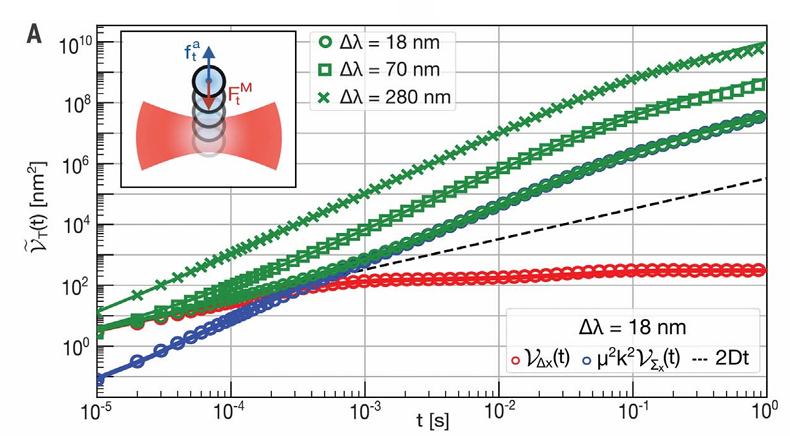
\includegraphics[width=8cm]{vsr_fig3a.png}  
  \end{center}
  \caption{ABP model}
\end{figure}

式 (\ref{vsr5}) を思い出せば,
\begin{equation}
  \mathcal{V} _{\Delta x} (t) + \mu^2 k^2 \mathcal{V} _{\Sigma_x} (t) = 2Dt + \tilde{\mathcal{S}}(t)
\end{equation}
であり,このグラフの縦軸は $\tilde{\mathcal{V}}_{T} = \mathcal{V} _{\Delta x} + \mu^2 k^2 \mathcal{V} _{\Sigma_x}$ である.
これは$\tilde{\mathcal{S}}(t) \neq 0$という理論的な予測と一致する.\\
\quad 最後にフィッティングの方法を述べる.このフィッティングによりモデルパラメーターと,$\sigma$を決定する.
式 (\ref{vsr5}) 
\begin{equation}
  \mathcal{V} _{\Delta x} (t) + \mu^2 k^2 \mathcal{V} _{\Sigma_x} (t) = 2Dt + \tilde{\mathcal{S}}(t)
\end{equation}
のうち,左辺は実験により直接的に求めることができる.
フィッティングのために,この式をラプラス変換し,つぎの等式を満たすようにパラメーターを決定する.
\begin{equation}
  \varepsilon (s) := \frac{\mathcal{V} _{\Delta x} (s) + \mu^2 k^2 \mathcal{V} _{\Sigma_x} (s) - \tilde{\mathcal{S}}(s)}{2D/s^2} = 1
\end{equation}
最もよくフィッティングされたものを $\varepsilon^{opt} (s)$ と書くことにする.\\
\quad つぎのグラフは SST model にてフィッティングした結果である.

\begin{figure}[H]
  \begin{center}  
  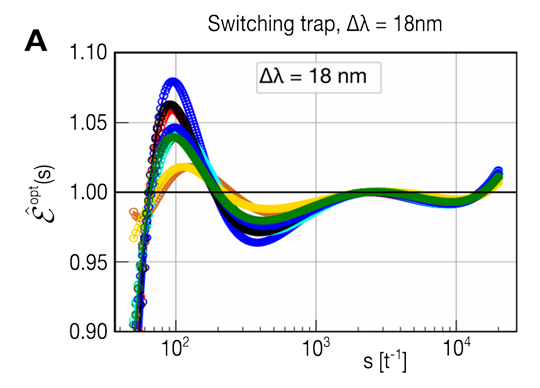
\includegraphics[width=8cm]{vsr_figs2a.png}  
  \end{center}
  \caption{SST model (fitting)}
\end{figure}

このフィッティングの結果,決定されたパラメーターがつぎの表である.

\begin{figure}[H]
  \begin{center}  
  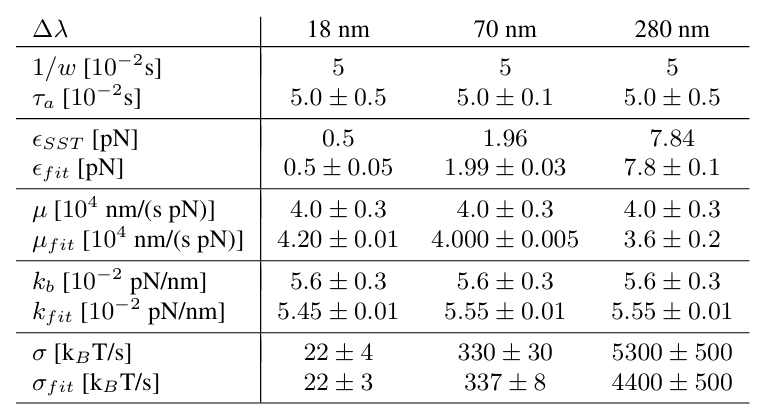
\includegraphics[width=10cm]{vsr_table1.png}  
  \end{center}
  \caption{SST model (fitting)}
\end{figure}

以上の方法により,$x(t)$ の情報のみから$\sigma $を決定することができた.

\newpage 
\section{RBC MODEL}
最後に Reduced VSR をヒト赤血球(RBC)に適用する.RBCは解糖系を通してグルコースをATPに代謝し,細胞膜のアクティブな振動を引き起こし,それに伴いエントロピーが生成する.\par 
この論文では3つの方法でRBCの実験を行った.1つは異なる強度の光トラップにより,膜に非特異的に結合したビーズを使ってRBCを機械的に引き延ばす方法.2つ目は先行研究(11)のデータを用いてRBC膜を機会的にセンシングする方法.3つ目は振動セグメントの追跡により,膜の輪郭の揺らぎを測定する方法である.\par 
ここでは figure S1 のように,見えない変数 $y(t)$ を設定した2層モデルを検討した.$x(t)$は測定することができる変数である.これらの変数はつぎの方程式を満たす.
\begin{equation}
  \dot{x}(t) = \mu_x (-k_b x(t) - k_{int}(x(t) - y(t)) + C_1) + \sqrt{2D_x} \eta^x (t) 
\end{equation}
\begin{equation}
  \dot{y}(t) = \mu_y (-k_c y(t) + k_{int}(x(t) - y(t)) + f^a (t) + C_2) + \sqrt{2D_y} \eta^y (t) 
\end{equation}
ここで $k_{i}$ は実効的な力の定数であり,$\mu_{i}, \eta_{i}$は移動度とホワイトノイズである.また,$C_i$は定数,$D_i$は $D_i = k_B T \mu_i$ である.$f^a (t)$は確率的なアクティブ力であって,つぎの関係を満たす.
\begin{equation}
  \dot{f}^a (t) = - \frac{f^a (t)}{\tau_a} + \sqrt{\frac{2 \epsilon^2}{\tau_a}} \eta^f (t)
\end{equation}
ただし,
\begin{equation}
  \ave{\eta^f (t) \eta^f (t')} = \delta (t - t')
\end{equation}

\newpage 
\section{補遺}
\subsection{エントロピー生成率(Langevin系)}
オーバーダンプなランジュバン方程式はつぎのように定義される.
\begin{equation}
  \gamma \frac{d \hat{x}}{dt} = F(\hat{x}, t) + \sqrt{2 \gamma T} \hat{\xi }(t)
\end{equation}
全系を注目している粒子と熱浴とすれば,全系でエネルギーが保存する.
熱力学第一法則を考え,仕事を熱浴から粒子へ行うものだと思えば,熱はその逆である.
すなわち
\begin{equation}
  d \hat{Q} = d \hat{x} \times_{\alpha } F_{\text{bath}} (\hat{x}, \hat{p}, t) = d \hat{x} \times_{\alpha } \qty( \frac{\gamma}{m} \hat{p} - \sqrt{2 \gamma T} \hat{\xi }(t) )
\end{equation}
となる.ここで $\times_{\alpha }$ は,我々が積のルールを決めなければならないことを明記している.
積のルールは熱力学の法則と整合するように決める.ここでは熱力学第一法則を考えることで決定する.
簡単のためにポテンシャルの無い状況を考え,散逸した熱が運動エネルギー変化に等しい場合を考える.
散逸する熱は
\begin{align}
  \hat{Q} &= \lim_{\Delta t \to 0} \sum_{n=0}^{N-1} \frac{1}{m} \qty( \hat{p} (t_n) + \alpha \qty[ - \frac{\gamma }{m} \hat{p}(t_n) \Delta t + \sqrt{2 \gamma T} \hat{\xi }_{\Delta t} (t_n) ] ) \\ 
  & \cdot \qty( \frac{\gamma }{m} \hat{p}(t_n) \Delta t - \sqrt{2 \gamma T} \hat{\xi }_{\Delta t} (t_n) ) \\
  &= \lim_{\Delta t \to 0} \sum_{n=0}^{N-1} \qty( \frac{\gamma }{m^2} \hat{p}(t_n)^2 \Delta t - \frac{2 \alpha \gamma T}{m} \Delta t ) + o(\Delta t)
\end{align}
であり,運動エネルギーの変化は
\begin{align}
   \lim_{\Delta \to 0} \sum_{n=0}^{N-1} \frac{1}{2m} \qty( \hat{p}(t_{n+1})^2 - \hat{p}(t_n)^2 ) \\
  &= \lim_{\Delta \to 0} \sum_{n=0}^{N-1} \frac{1}{2m} \qty( \qty[ \hat{p}(t_{n}) - \frac{\gamma }{m} \hat{p}(t_n) \Delta t + \sqrt{2 \gamma T} \hat{\xi }_{\Delta t}(t_n)] - \hat{p}(t_n)^2) \\
  &= \lim_{\Delta \to 0} \sum_{n=0}^{N-1} \frac{1}{2m} \qty( -2 \frac{\gamma}{m} \hat{p}(t_n)^2 \Delta t + 2 \gamma T \Delta t )
\end{align}
となる.両者が等しいためには $\alpha = \frac{1}{2}$ が必要であり,それは Stratonovich 積である.

\subsection{アクティブノイズとエントロピー生成の関係}
ここでは簡単なモデルに対してアクティブノイズをかけることでエントロピー生成が増加することを確認する. 
ここでいうアクティブノイズは,つぎのようなものである.
\begin{equation}
  \ave{f^a (t)} = 0
\end{equation}
\begin{equation}
  \ave{f^a (t) f^a (s)} = \epsilon^2 \exp( - \frac{|t-s|}{\tau_a} )
\end{equation}
ただし,$\tau_a$ は時間相関長である.\\
\quad まずは調和ポテンシャルによりトラップされた水中の粒子に対してアクティブノイズをかける.
EOMは
\begin{equation}
  \dot{x}(t) = -k \mu x(t) + \sqrt{2D} \eta(t) + \mu f^a (t)
\end{equation}
であって,excess varianceは,つぎのように計算される.
\begin{align}
  \tilde{\mathcal{S}}(t) &= 2\mu^2 \int_0^t ds \int_0^s du \ave{ f^a(u) f^a(0) } \\
  &= 2 \epsilon^2 \mu^2 \tau_a \qty[ t - \tau_a \qty(1- \exp(-\frac{t}{\tau_a})) ]
\end{align}
このときの $\sigma$ を $\sigma_a$ とする.\\
\quad これに対し,アクティブノイズをかけない場合について考えると,EOMは
\begin{equation}
  \dot{x}(t) = -k \mu x(t) + \sqrt{2D} \eta(t)
\end{equation}
である.すなわち $\mu = 0$なので,
\begin{align}
  \tilde{\mathcal{S}}(t) &= 0
\end{align}
となり,このときの $\sigma$を $\sigma_0$ とする.
$\tilde{\mathcal{S}}(t)$ の大きさを比較することで,必ず $\sigma_a > \sigma_0$ となる.

\subsection{キネシンのモデル(提案)}
キネシンにReduced-VSRを適用するために,つぎのようなモデルを考える.

\begin{figure}[H]
  \begin{center}
  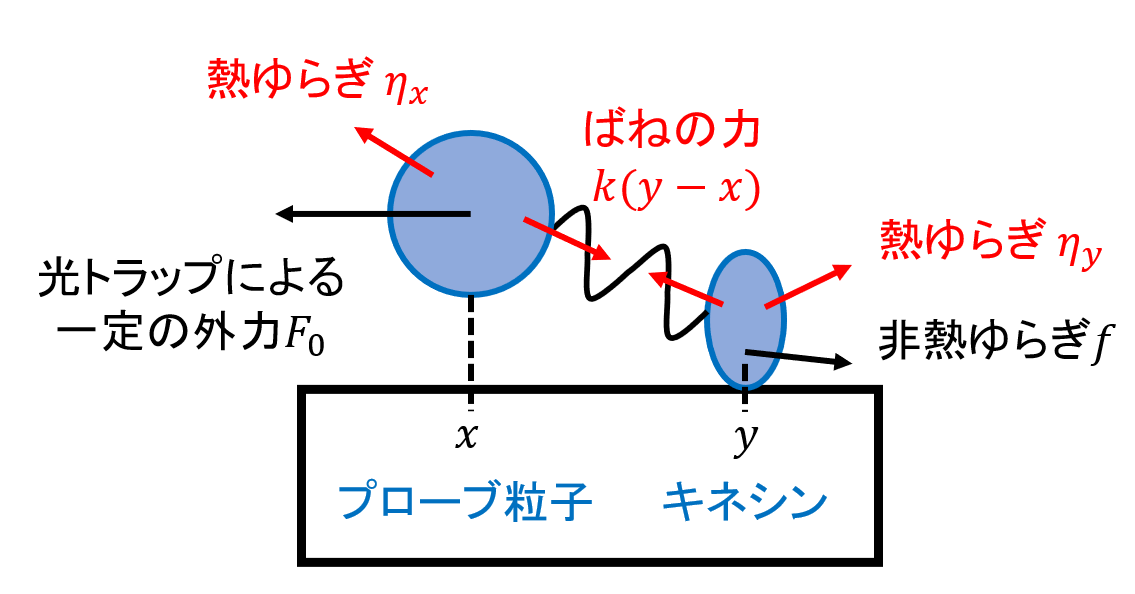
\includegraphics[width=10cm]{kinesine_suggest.png}
  \end{center}
  \caption{提案するキネシンのモデル}
\end{figure}

この場合のオーバーダンプなランジュバン方程式は,つぎの2式である.
\begin{equation}
  \dot{x}(t) = \mu_x k (y(t) - x(t)) + F_0 + \sqrt{2D_x} \eta_x (t)
\end{equation}
\begin{equation}
  \dot{y}(t) = - \mu_y k (y(t) - x(t)) + f(t) + \sqrt{2D_y} \eta_y (t)
\end{equation}
いくつかの注意を以下に列挙する.
\begin{itemize}
  \item $x(t)$ はプローブの座標で,$y(t)$ はキネシンの座標である.前者は測定可能だが,後者は測定できない.
  \item $F_0$ は光トラップによる一定の外力
  \item $\ave{\eta_i (t) \eta_j (s)} = \delta_{ij} \delta (t-s)$ であり,熱ゆらぎの大きさは $\sqrt{2D_i}$ に現れる.
  \item $\ave{f(t) f(s)} = \epsilon^2 \exp( - \frac{|t-s|}{\tau_a} )$ を満たすとし,$\tau_a, \epsilon$ はフィッテングにより決定する.
  \item $\mu_i = \gamma_i^{-1}$
  \item $k$ はプローブとキネシンで共通となる.
  \item プローブにかかる非熱ゆらぎ $f$ は,一定の外力 $F_0$ より十分小さいとした.
  \item 光トラップはキネシンには当てないため,$F_0$ が入らない.
\end{itemize}

\subsection{線形応答理論}
注目系の状態が逆温度 $\beta = (k_B T)^{-1}$ の平衡状態にあるとし,時刻 $t = t_0$ で注目系に外場を印加する.
そうして $t = \tau $ で演算子 $A$ の平均値を見る.
このとき全系のハミルトニアン $H$ は摂動項 $-BF(t)$ を加えたものであり,
\begin{equation}
  H_{\text{tot}} = H - BF(t)
\end{equation}
初期時刻 $t = t_0$ では,系は無摂動ハミルトニアン $H$ の平衡状態にある.
すなわち $\mathbf{\pi } = \frac{e^{-\beta H}}{\Tr e^{-\beta H}}$ である.
この状態から摂動を加え,演算子 $A$ の応答を見ていく.
注目系の状態が逆温度 $\beta = (k_B T)^{-1}$ の平衡状態にあるとし,時刻 $t = t_0$ で注目系に外場を印加する.
そうして $t = \tau $ で演算子 $A$ の平均値を見る.
このとき全系のハミルトニアン $H$ は摂動項 $-BF(t)$ を加えたものであり,
\begin{equation}
  H_{\text{tot}} = H - BF(t)
\end{equation}
初期時刻 $t = t_0$ では,系は無摂動ハミルトニアン $H$ の平衡状態にある.
すなわち $\mathbf{\pi } = \frac{e^{-\beta H}}{\Tr e^{-\beta H}}$ である.
この状態から摂動を加え,演算子 $A$ の応答を見ていく.


\newpage 
\section{参考文献}
[1] Dieterich, E., et al. "Single-molecule measurement of the effective temperature in non-equilibrium steady states." Nature Physics 11.11 (2015): 971-977.

\end{document}